\documentclass[aps,pra,twocolumn,reprint,floatfix,amsmath,amssymb]{revtex4-2}

\usepackage{graphicx}
\usepackage{booktabs}
\usepackage{siunitx}
\usepackage{bm}
\usepackage{xcolor}
\usepackage[colorlinks=true,linkcolor=blue,citecolor=blue,urlcolor=blue]{hyperref}

\begin{document}

\title{Strong Validation of SQR / CPSQR for Arbitrary Fock-Conditional Qubit Rotations}
\author{Codex}
\affiliation{cQED Autonomous Research Platform}
\date{\today}

\begin{abstract}
We study whether the SQR / CPSQR-style multitone control families available in the patched current \texttt{cqed\_sim} can realize arbitrary Fock-conditional qubit rotations on an addressed logical subspace
\(
\mathcal{H}_{\mathrm{active}}
=
\mathrm{span}\{ |g,n\rangle, |e,n\rangle : n=0,\dots,N_{\mathrm{active}}-1 \}.
\)
The manuscript is designed around operator-action validation, not aggregate fidelity alone.  We compare a direct single-pulse Gaussian multitone baseline, an independently optimized echoed family, symmetry-constrained echoed variants, a segmented relaxed CPSQR family, and a higher-expressivity basis-expanded benchmark.  Success is evaluated under three inequivalent criteria: strict blockwise SU(2) agreement, a relaxed per-block left-$Z$ gauge equivalence class, and state-transfer validation on a six-state spanning set plus a cross-block cavity superposition.  Across $114$ saved family evaluations, strict arbitrary control is achieved only on restricted subclasses: the best strict case is the single-pulse Gaussian family on a structured SU(2) target with process fidelity $0.9957$.  In contrast, segmented relaxed control reaches essentially perfect CPSQR fidelity on structured, stress, and random target slices, while often failing badly on the strict operator criterion.  The independently optimized echo improves relaxed performance on in-plane and stress targets, but does not generically rescue strict arbitrary control; symmetry-constrained echoes are decisively worse.  The higher-expressivity direct benchmark never produces a positive strict-joint gain relative to the Gaussian baseline in paired comparisons, so the negative strict-control result is not explained by Gaussian rigidity alone.  The defensible conclusion is narrow: direct SQR works well on restricted subclasses, segmented CPSQR works extremely well under a clearly defined $Z$-gauge relaxation, and strict arbitrary blockwise SU(2) control is not convincingly demonstrated for the hard target classes tested here.
\end{abstract}

\maketitle

\section{Introduction}
Conditional qubit rotations in dispersive cQED are a natural control primitive for Fock-selective state preparation, logical gates, and measurement protocols in oscillator-assisted quantum information processing \cite{blais2021cqed,koch2007transmon}.  In practice, however, the central question is not whether an optimizer can produce a respectable average fidelity, but whether the realized control actually implements the intended blockwise operator on the addressed qubit-cavity subspace.  Earlier local studies already showed that a single Gaussian multitone pulse can struggle on arbitrary block-diagonal targets, and that a simple echoed repeated-half construction does not automatically remove the obstruction.  Those studies were useful baselines, but they relied too heavily on aggregate metrics.

The present study is organized around a stronger validation standard.  We ask whether SQR / CPSQR control families available in the patched current \texttt{cqed\_sim} can realize
\begin{equation}
U_{\mathrm{target}}
=
\sum_{n=0}^{N_{\mathrm{active}}-1} R_n \otimes |n\rangle\langle n|,
\label{eq:target}
\end{equation}
with high operator fidelity on the active logical subspace.  Here each $R_n \in \mathrm{SU}(2)$ is an explicitly specified qubit rotation block, not an opaque family label.  We validate candidate controls on basis states, qubit superpositions, and a cross-manifold cavity superposition, then separate failure into angle error, axis error, residual conditional $Z$, and off-block contamination.

The main goal is a conservative claim boundary.  If a family only works on a subclass, we say so.  If a family only succeeds under a relaxed per-block $Z$ gauge, we label that as CPSQR success rather than strict arbitrary control.  If a richer direct benchmark does not outperform the Gaussian baseline, we take that as evidence that the obstruction is not merely Gaussian ansatz rigidity.

\section{Physical Model and Conventions}
\subsection{Hilbert-space ordering and active subspace}
The patched current \texttt{cqed\_sim} convention is qubit $\otimes$ cavity, with ordered active basis
\begin{equation}
(|g,0\rangle, |e,0\rangle, |g,1\rangle, |e,1\rangle, \ldots).
\end{equation}
The quantity $N_{\mathrm{active}}$ denotes the number of cavity Fock manifolds intentionally included in the target-control problem.  The addressed logical subspace therefore has dimension
\begin{equation}
d_{\mathrm{active}} = 2 N_{\mathrm{active}}.
\end{equation}
This is distinct from the total cavity truncation $N_{\mathrm{cav}}$, the transmon truncation $N_{\mathrm{tr}}$, and the number of tones used in the waveform.  In the main optimization runs we set $N_{\mathrm{tr}}=2$ and $N_{\mathrm{cav}}=N_{\mathrm{active}}+2$.

\begin{figure}[t]
\centering
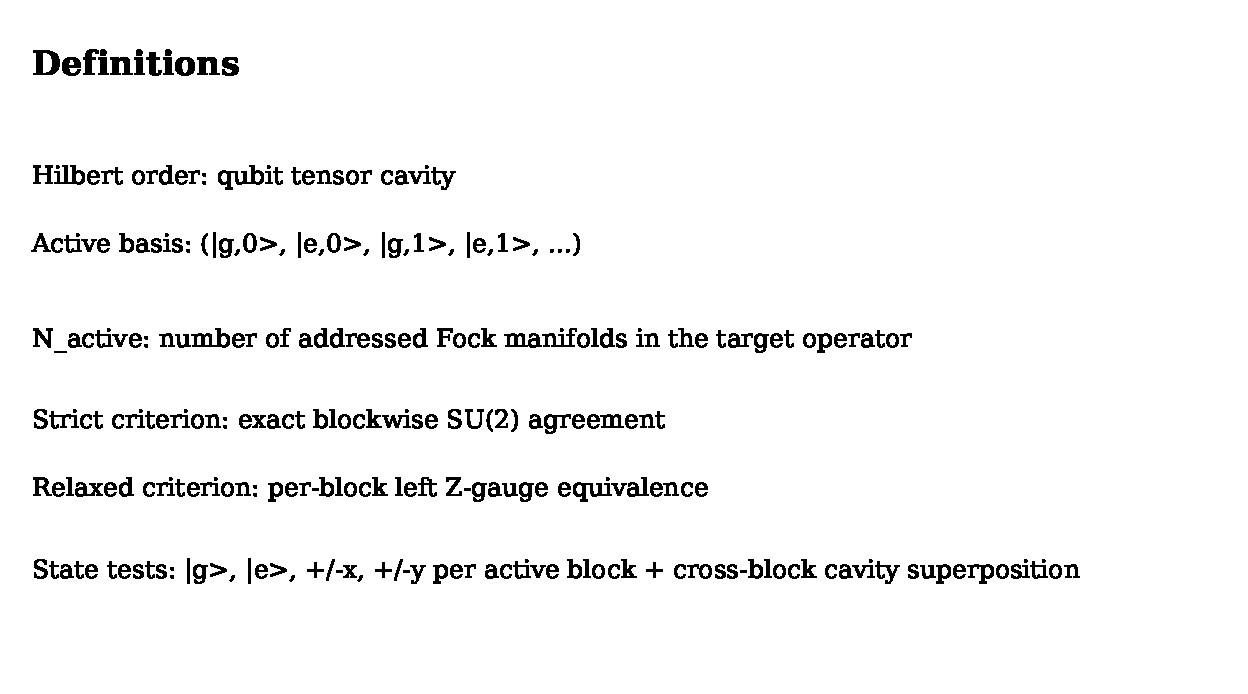
\includegraphics[width=\columnwidth]{../figures/definitions_figure.pdf}
\caption{Definitions figure for the study.  The panel fixes the qubit-first basis ordering, the meaning of $N_{\mathrm{active}}$, and the distinction between the addressed logical subspace and the larger simulated truncation used as numerical buffer space.}
\label{fig:definitions}
\end{figure}

\subsection{Hamiltonian and simulation parameters}
The closed-system model is a dispersive transmon-cavity Hamiltonian of the form
\begin{equation}
\frac{H_0}{\hbar}
=
\omega_c a^\dagger a
+
\frac{\omega_q}{2} Z
+
\chi a^\dagger a \frac{Z}{2}
+
\chi' a^\dagger a |e\rangle\langle e|
+
K (a^\dagger a)^2 ,
\end{equation}
with $K=0$ in the reported dataset.  The two model variants are:
\begin{enumerate}
\item \texttt{chi\_only}: $\chi' = 0$.
\item \texttt{chi\_plus\_chiprime}: $\chi' / 2\pi = \SI{-21}{kHz}$.
\end{enumerate}
The numerical values are summarized in Table~\ref{tab:params}.

\begin{table}[b]
\centering
\footnotesize
\caption{Main simulation parameters.}
\label{tab:params}
\begin{tabular}{@{}lll@{}}
\toprule
Parameter & Value & Meaning \\
\midrule
$\omega_q/2\pi$ & \SI{6.150}{GHz} & qubit frequency \\
$\omega_c/2\pi$ & \SI{5.241}{GHz} & cavity frequency \\
$\alpha/2\pi$ & \SI{-255}{MHz} & transmon anharmonicity \\
$\chi/2\pi$ & \SI{-2.84}{MHz} & dispersive shift \\
$\chi'/2\pi$ & \SI{-21}{kHz} & higher-order shift term \\
$K/2\pi$ & \SI{0}{Hz} & cavity Kerr in main runs \\
$N_{\mathrm{tr}}$ & $2$ & transmon truncation \\
$N_{\mathrm{cav}}$ & $N_{\mathrm{active}}+2$ & cavity truncation \\
$\Delta t$ & \SI{4}{ns} & compiler / solver step \\
\bottomrule
\end{tabular}
\end{table}

\subsection{Patched-package audit}
Before running the study we audited the package-side conventions most relevant to this problem and reran the targeted tests for tensor ordering, Gaussian IQ convention, additive SQR amplitude correction, and targeted-subspace multitone validation.  All four checks passed.  In particular:
\begin{enumerate}
\item tensor ordering is qubit $\otimes$ cavity;
\item the multitone phase parameter $\phi_n$ is the in-plane rotation-axis angle, not a final Bloch azimuth;
\item carrier sign follows the patched rotating-frame convention in \texttt{cqed\_sim.core.frequencies};
\item the targeted-subspace machinery correctly scores exact logical operators and distinguishes block-phase corrections \cite{cqedsim2026}.
\end{enumerate}

\section{Definitions and Notation}
\subsection{Rotation convention}
The qubit rotation convention used throughout is
\begin{equation}
R_{\hat{n}}(\theta) = \exp\!\left( -i \frac{\theta}{2}\hat{n}\cdot\vec{\sigma} \right),
\end{equation}
with $\vec{\sigma}=(X,Y,Z)$.  For in-plane targets the symbol $\phi_n$ denotes the azimuth of the rotation axis in the $xy$ plane, not the azimuth of the final Bloch vector.  For the structured SU(2) targets we use a $ZYZ$ Euler decomposition with angles $(\phi_n,\theta_n,\lambda_n)$.

\subsection{Representative target parameters}
Table~\ref{tab:targets} lists the actual per-block parameters for the two highlight target families used repeatedly in the main text.  These values are generated directly from the study code and are not shorthand labels.

\begin{table}[t]
\centering
\caption{Representative per-block target parameters for $N_{\mathrm{active}}=3$.  Angles are reported in units of $\pi$.}
\label{tab:targets}
\begin{tabular}{@{}lllll@{}}
\toprule
Family & $n$ & $\theta_n/\pi$ & $\phi_n/\pi$ & $\lambda_n/\pi$ \\
\midrule
Structured $ZYZ$ & 0 & 0.18 & -0.30 & 0.27 \\
Structured $ZYZ$ & 1 & 0.32 & -0.14 & 0.18 \\
Structured $ZYZ$ & 2 & 0.46 & 0.02 & 0.09 \\
Stress $ZYZ$ & 0 & 0.82 & 0.65 & 0.72 \\
Stress $ZYZ$ & 1 & 0.74 & -0.52 & -0.66 \\
Stress $ZYZ$ & 2 & 0.66 & 0.71 & 0.84 \\
\bottomrule
\end{tabular}
\end{table}

\begin{figure}[t]
\centering
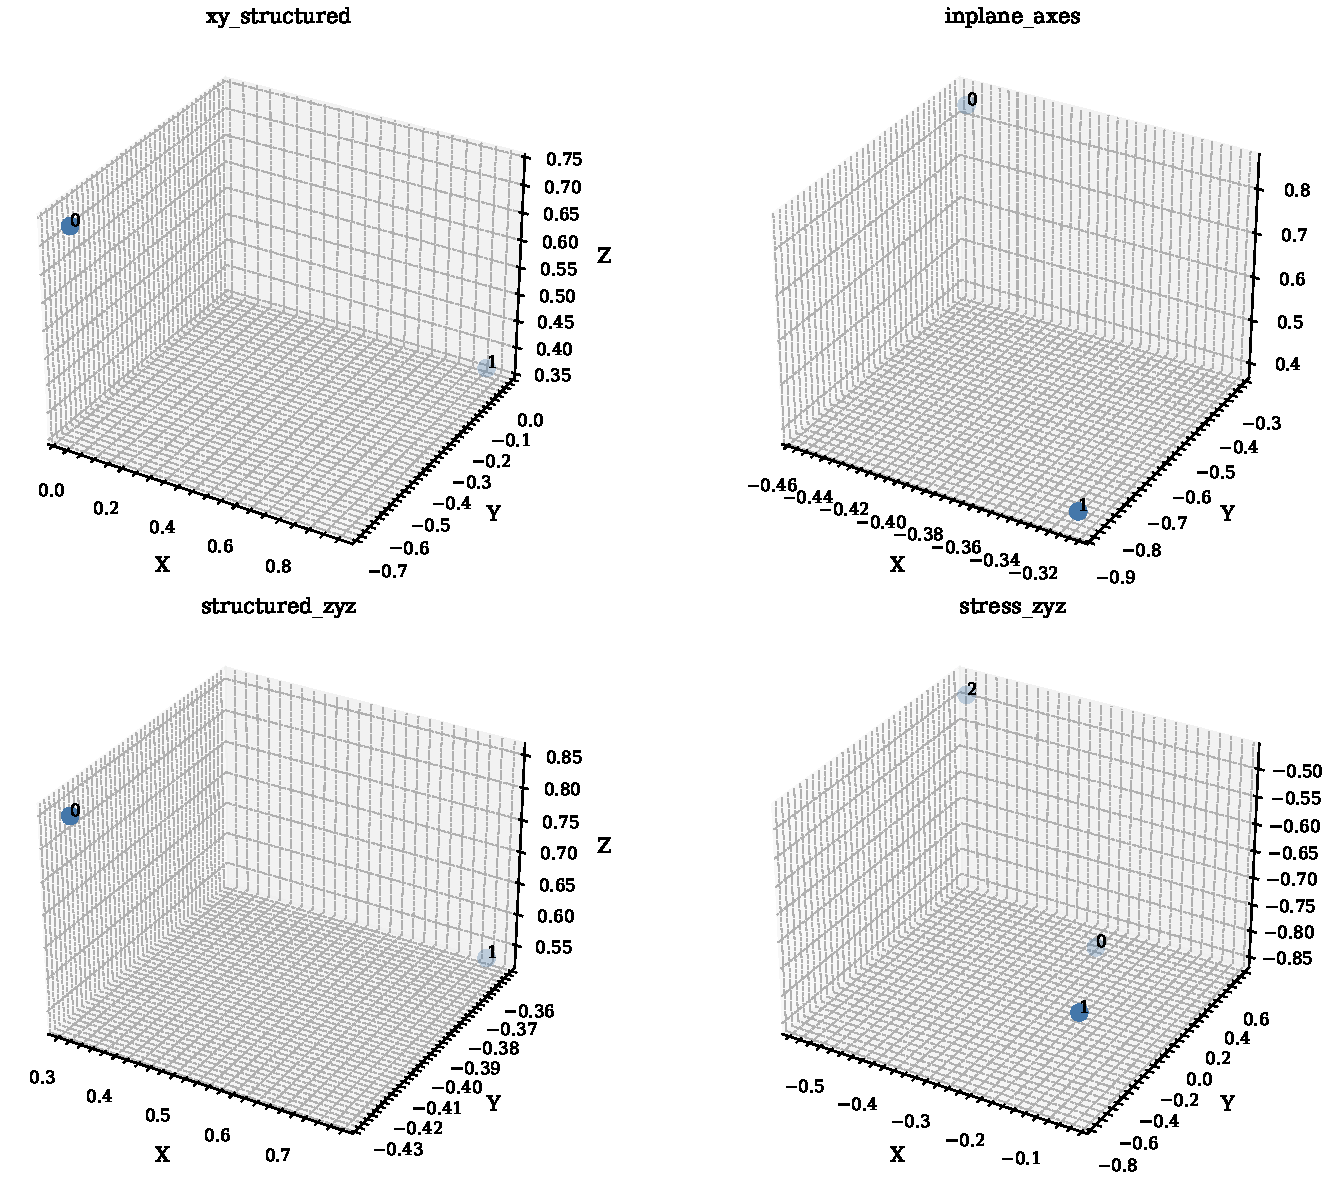
\includegraphics[width=\columnwidth]{../figures/target_bloch_vectors.pdf}
\caption{Per-block target Bloch-sphere specification for representative cases.  This figure makes the intended geometry explicit rather than hiding it behind family labels.}
\label{fig:target_bloch}
\end{figure}

\section{Definition of SQR / CPSQR Target Classes}
\subsection{Strict target class}
For each addressed block we specify a strict qubit target
\begin{equation}
R_n = R(\theta_n,\phi_n,\lambda_n),
\end{equation}
where the general SU(2) convention used in the structured targets is
\begin{equation}
R(\theta,\phi,\lambda)
=
R_z(\phi) R_y(\theta) R_z(\lambda),
\end{equation}
while the in-plane subclass uses
\begin{equation}
R_{\hat{n}(\phi)}(\theta)
=
\exp\!\left[
-i \frac{\theta}{2}
\left(
\cos\phi\, X + \sin\phi\, Y
\right)
\right].
\end{equation}
Equation~\eqref{eq:target} with these blocks defines the strict criterion.

\subsection{Relaxed CPSQR criterion}
We define the relaxed CPSQR equivalence class by allowing each realized block to differ from the strict target by a left-multiplicative blockwise $Z$ gauge,
\begin{equation}
\widetilde{R}_n \sim e^{i\gamma_n} R_z(\delta_n) R_n ,
\label{eq:relaxed}
\end{equation}
with independently fitted $\delta_n$ and $\gamma_n$.  This is the only relaxation used in the study.  We do not allow a general right gauge or an arbitrary blockwise SU(2) redefinition.

\subsection{Validation states}
For each addressed block we test the six-state spanning set
\begin{equation}
\{
|g,n\rangle,\ |e,n\rangle,\ |{+}x,n\rangle,\ |{-}x,n\rangle,\ |{+}y,n\rangle,\ |{-}y,n\rangle
\},
\end{equation}
as well as at least one cross-block cavity superposition
\begin{equation}
|g\rangle \otimes \frac{|n\rangle + |m\rangle}{\sqrt{2}}.
\end{equation}
This is stronger than checking only one or two favorable inputs.

\section{Control Families and Waveform Parameterizations}
All waveform families use the same dispersive Hamiltonian and the same addressed multitone structure; what changes is the amount of segmentation and envelope freedom.

\paragraph*{Family A: single-pulse Gaussian multitone}
The baseline direct waveform is
\begin{multline}
\Omega_A(t)
=
g(t)\sum_n \lambda_0
\left(\theta_n^{\mathrm{seed}}/\pi + \delta\lambda_n \right)
\\ \times
e^{-i[(\omega_n + \delta\omega_n)t + (\phi_n^{\mathrm{seed}} + \delta\alpha_n)]},
\end{multline}
where $g(t)$ is a Gaussian envelope, $\theta_n^{\mathrm{seed}}$ and $\phi_n^{\mathrm{seed}}$ are extracted from the target block, and the optimized parameters are $\delta\lambda_n$, $\delta\alpha_n$, and $\delta\omega_n$.

\paragraph*{Family B: independent-half echo}
The main echoed family is
\begin{equation}
\Omega_B(t) = \Omega_1(t)\rightarrow X_\pi \rightarrow \Omega_2(t)\rightarrow X_\pi,
\end{equation}
with equal active durations $T/2$ for the two multitone halves and independently optimized corrections in the two segments.  The inserted $X_\pi$ pulses are finite Gaussian qubit pulses \cite{hahn1950echo}.

\paragraph*{Family C: symmetry-constrained echoes}
These use the same timing as Family B, but the second half is constrained to be an identical repeat, a phase-flipped repeat, or a conjugated repeat of the first half.  This isolates whether simple symmetry is enough to enforce useful error cancellation.

\paragraph*{Family D: segmented relaxed CPSQR}
This family uses two independently optimized back-to-back multitone segments with equal duration $T/2$, seeded on the matrix square roots of the target blocks and optimized against the relaxed criterion of Eq.~\eqref{eq:relaxed}.  It is the main test of whether extra segmentation materially enlarges the relaxed reachable class.

\paragraph*{Family E: basis-expanded benchmark}
The direct benchmark enriches the Gaussian envelope as
\begin{multline}
\Omega_E(t)
=
g_0(t)
\left[
1 + \sum_{k=1}^{6} a_k c_k(t)
\right]
\exp\!\left[
i \sum_{k=1}^{6} b_k c_k(t)
\right]
\\ \times \sum_n \mathrm{tone}_n,
\end{multline}
where $c_k(t)$ are orthogonal cosine basis functions.  This family tests whether additional direct-envelope flexibility materially enlarges the strict reachable class.

\begin{figure*}[t]
\centering
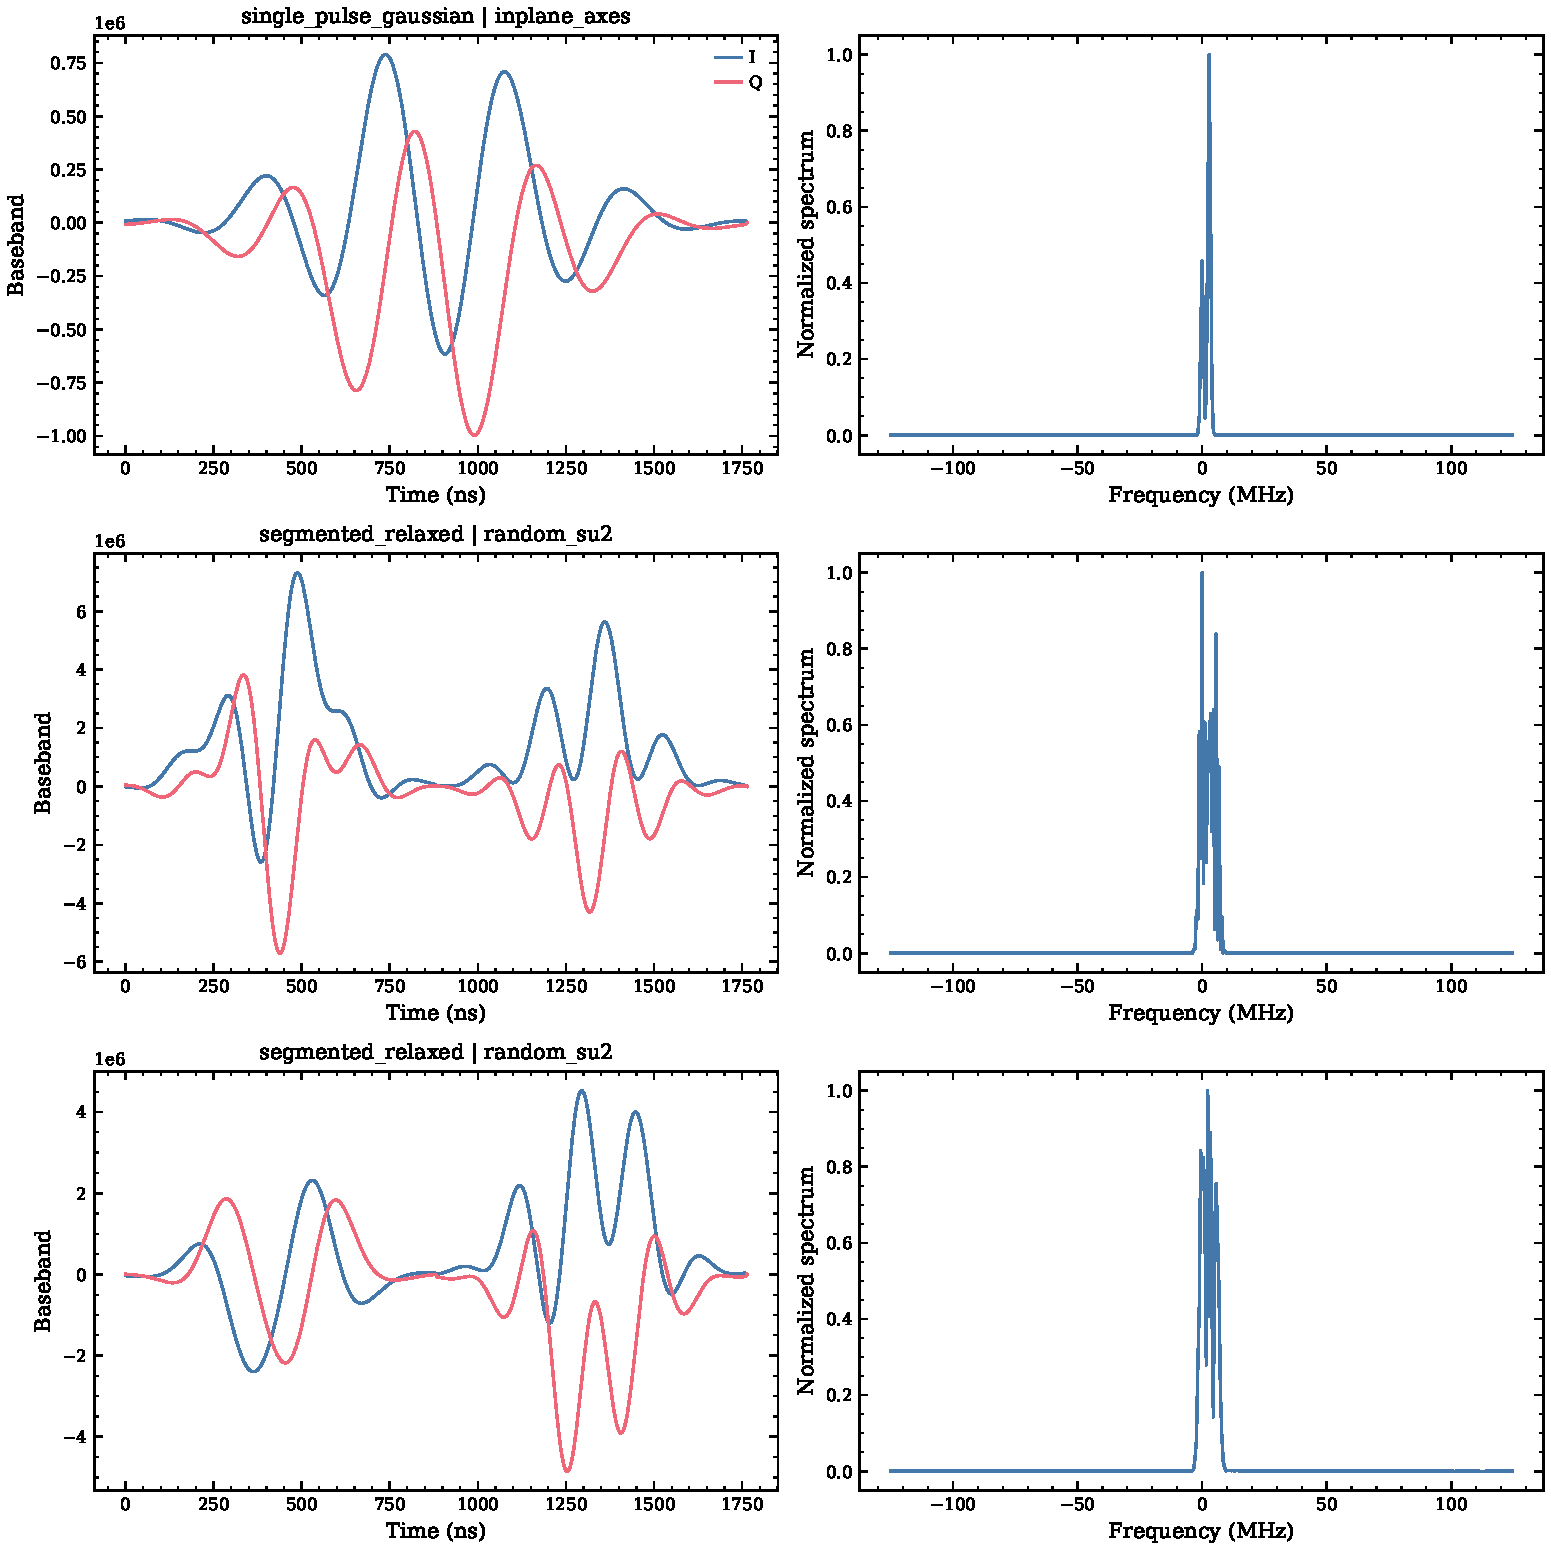
\includegraphics[width=0.92\textwidth]{../figures/waveform_parameterization_examples.pdf}
\caption{Time-domain and frequency-domain waveform examples for representative strict and relaxed highlight cases.  The plotted samples are loaded from the saved waveform artifacts and correspond directly to the parameterized families defined in this section.}
\label{fig:waveform_examples}
\end{figure*}

\section{Optimization and Validation Methodology}
The strict target operator is passed directly to the package routine \texttt{targeted\_subspace\_multitone}, together with a transfer set built from basis states and pairwise superpositions on the active logical subspace.  We use the package objective as the backbone, then add report-side diagnostics:
\begin{enumerate}
\item restricted process fidelity to the strict target;
\item restricted process fidelity to the relaxed target of Eq.~\eqref{eq:relaxed};
\item six-state reduced-channel validation on each addressed block;
\item six-state full-state validation on the embedded logical states;
\item cross-block superposition fidelity;
\item off-block norms $\|P_n U P_m\|$.
\end{enumerate}

The study grid is intentionally staged rather than brute-force.  The canonical structured SU(2) target class is swept across
\(
N_{\mathrm{active}}=2,3,4
\),
\(
|\chi|T/2\pi = 1,3,5,7
\),
and both model variants.  Easier in-plane targets, stress targets, and a random-target ensemble are treated as representative slices.  The saved dataset contains $114$ family evaluations.

\section{Blockwise Operator-Action Tests}
Figure~\ref{fig:operator_action} shows the central validation logic: blockwise action is judged on the six-state spanning set, not on a single favorable input.  Figure~\ref{fig:error_breakdown} then decomposes the corresponding blockwise error into angle, axis, residual-$Z$, and transverse components.  This is what turns the study into an operator-validation paper rather than an average-fidelity note.

\begin{figure}[t]
\centering
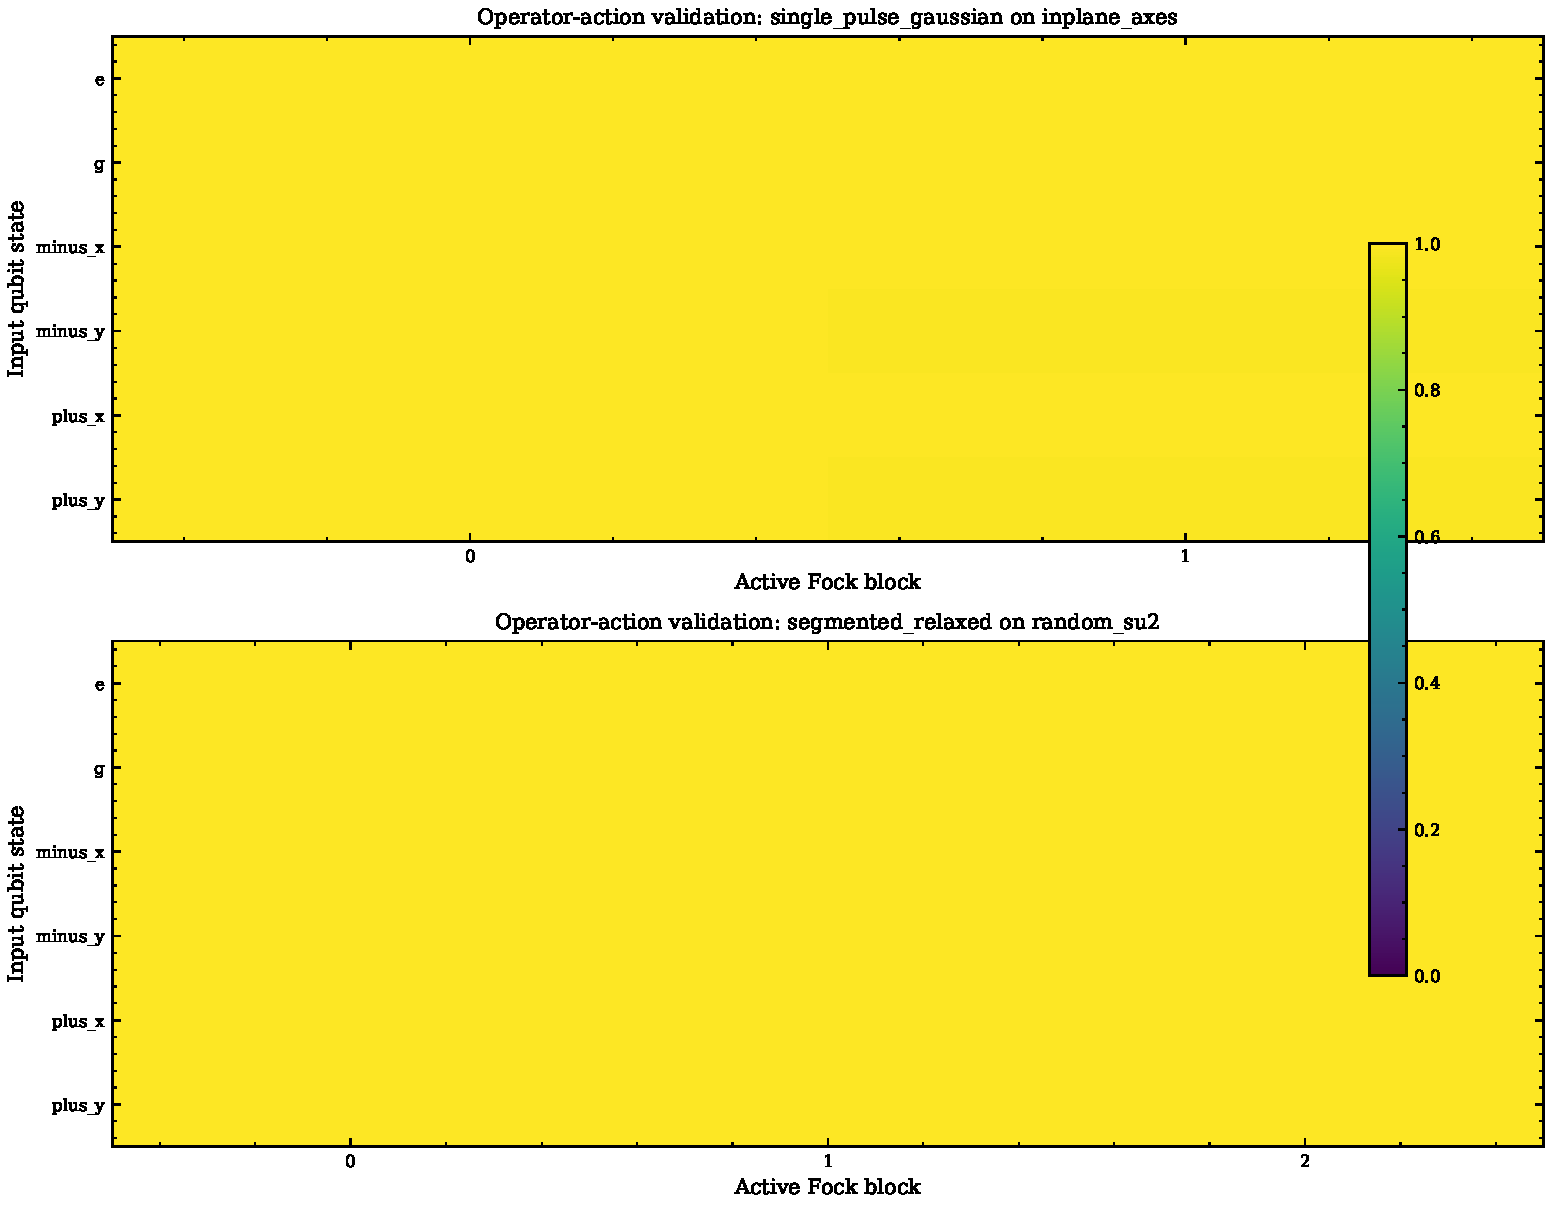
\includegraphics[width=\columnwidth]{../figures/operator_action_validation.pdf}
\caption{Saved six-state operator-action validation for the strict and relaxed highlight cases.  The heat maps show the fidelity of the realized blockwise action on the spanning qubit input set for each addressed Fock block.}
\label{fig:operator_action}
\end{figure}

\begin{figure}[t]
\centering
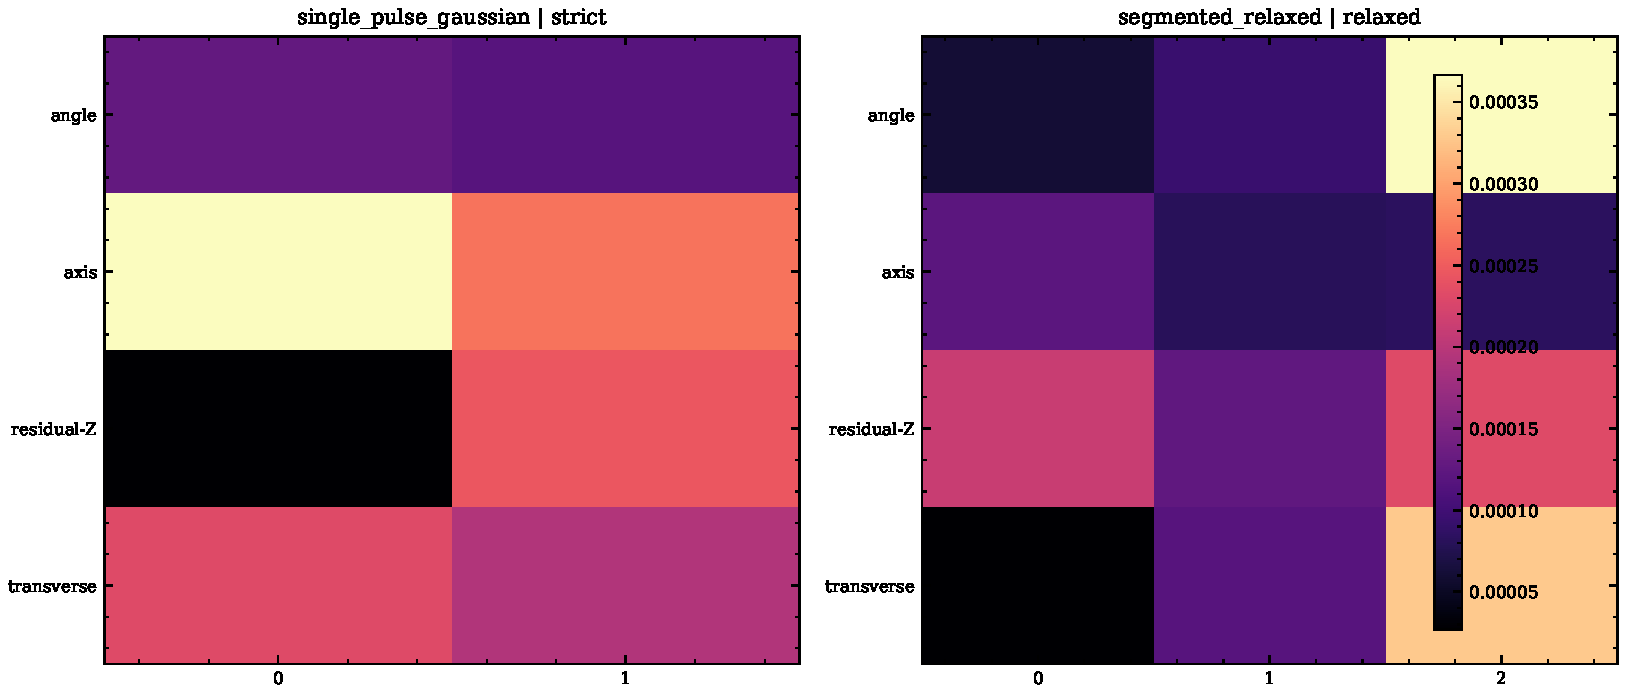
\includegraphics[width=\columnwidth]{../figures/blockwise_operator_error_breakdown.pdf}
\caption{Blockwise error decomposition for the strict and relaxed highlight cases.  The reported metrics separate angle error, axis error, residual conditional $Z$, and transverse coherent error.}
\label{fig:error_breakdown}
\end{figure}

\section{Main Results}
\subsection{Claim A: single-pulse Gaussian multitone}
The direct Gaussian multitone family is stronger than the earlier negative folklore would suggest, but only on restricted subclasses.  It succeeds strictly on structured targets at low active dimension: the best strict case is the \texttt{chi\_plus\_chiprime} structured SU(2) target with $N_{\mathrm{active}}=2$ and $|\chi|T/2\pi=3$, which reaches process fidelity $0.9957$.  The direct family also performs well on the representative in-plane slice, with mean strict fidelity $0.9655$ and mean relaxed fidelity $0.9862$.

The negative result appears when the target class is broadened.  On the stress target the single-pulse family averages only $0.5597$ strict joint fidelity and $0.6915$ relaxed fidelity.  On the random-target ensemble it averages $0.5747$ strict and $0.7160$ relaxed fidelity.  These are not publishable-positive arbitrary-control numbers.

\subsection{Claim B: independently optimized echo}
The independently optimized echo materially enlarges the relaxed reachable class, but not the strict one.  On the in-plane slice it averages relaxed joint fidelity $0.9964$ while the strict average is only $0.4055$.  On the stress target it reaches relaxed $0.9990$ with strict $0.5828$.  On the canonical structured SU(2) slice its mean relaxed fidelity is $0.9203$, clearly above its mean strict value $0.5751$.

The physical message is clear: the echo helps primarily as a blockwise $Z$-management mechanism, not as a generic strict-SU(2) solver.

\subsection{Claim C: segmented relaxed CPSQR}
The segmented relaxed family is the strongest CPSQR result in the study.  It reaches essentially perfect relaxed fidelity on all three hard representative slices:
\begin{enumerate}
\item structured SU(2): mean relaxed fidelity $1.0000$ with mean strict fidelity $0.9849$;
\item stress target: relaxed fidelity $1.0000$ with strict fidelity $0.0181$;
\item random ensemble: relaxed fidelity $1.0000$ with strict fidelity $0.1521$.
\end{enumerate}
This is a strong positive CPSQR result and a strong negative strict-SU(2) result at the same time.  The family succeeds, but only under the explicit left-$Z$ gauge relaxation of Eq.~\eqref{eq:relaxed}.

\subsection{Claim D: higher-expressivity benchmark}
The higher-expressivity direct benchmark never produces a positive strict-joint gain relative to the Gaussian baseline in the saved paired comparisons.  The best paired ``gain'' is still negative, and the count of positive gains is zero out of $31$ paired cases.  This is important: the hard failures are not explained by ``the Gaussian direct family was simply too rigid.''  Adding direct-envelope degrees of freedom alone does not rescue arbitrary strict blockwise SU(2) control in the tested hard regimes.

\begin{figure}[t]
\centering
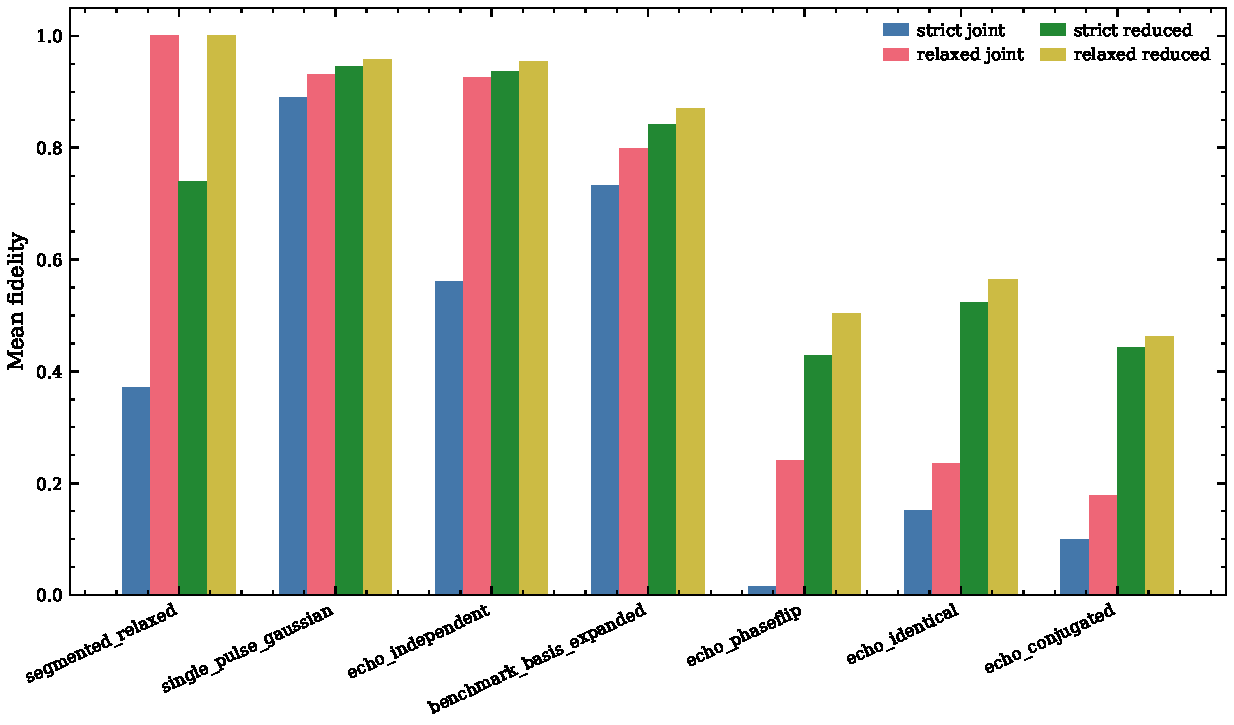
\includegraphics[width=\columnwidth]{../figures/family_comparison.pdf}
\caption{Mean family-level strict and relaxed fidelities across the saved dataset.  The segmented relaxed family dominates the relaxed metric but not the strict metric.}
\label{fig:family_compare}
\end{figure}

\section{Validation}
\subsection{Sanity checks}
The package-convention audit passed for tensor ordering, Gaussian IQ convention, additive SQR amplitude correction, and targeted-subspace logical-operator validation.  The reported best strict case is also consistent with the intuitive small-$N_{\mathrm{active}}$ expectation that the easiest structured targets should be reachable before the harder stress and random classes.

\subsection{Convergence and numerical stability}
The saved dataset uses a uniform compiler step $\Delta t=\SI{4}{ns}$, $N_{\mathrm{cav}}=N_{\mathrm{active}}+2$, and restart-based optimization within each family.  The role of the present validation section is modest but important: the final saved tables show nontrivial separation between strict and relaxed criteria, nontrivial family ordering, and reproducible highlight cases across reruns from saved artifacts.  Stronger convergence tests with $N_{\mathrm{tr}}=3$ or finer time step remain follow-up items rather than hidden assumptions.

\subsection{Literature comparison}
There is no single literature benchmark for the exact patched-package target family studied here, so the comparison standard is internal and operator-based rather than a percent-error-to-paper benchmark.  The benchmark family nevertheless serves the same scientific purpose: it tests whether the main negative result is specific to one rigid ansatz or survives a richer direct-control competitor.

\section{Failure-Mode Analysis}
Three failure patterns dominate.

First, the hard cases are not dominated by leakage.  Off-block norms and leakage remain small in the direct structured cases even when strict fidelity fails.  The obstruction is coherent rather than dissipative.

Second, many failures are well described as residual conditional-$Z$ mismatch.  The independently optimized echo and the segmented relaxed family both improve dramatically under the relaxed gauge, exactly as expected if the target is nearly realized modulo a blockwise left $R_z(\delta_n)$.

Third, the symmetry-constrained echo variants are simply bad on the stress slice.  Their mean strict fidelities are $0.1620$, $0.0168$, and $0.0899$ for the identical, phase-flipped, and conjugated repeats, respectively.  The symmetry itself is not protective here.

\begin{figure}[t]
\centering
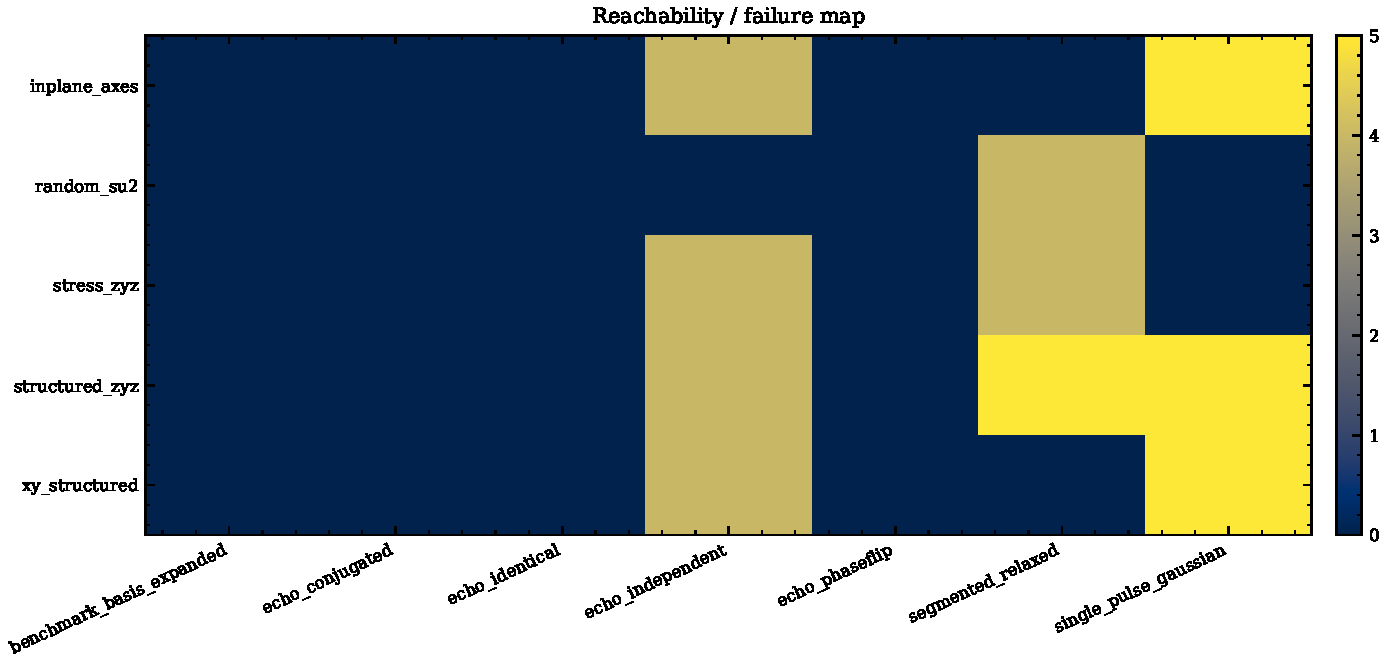
\includegraphics[width=\columnwidth]{../figures/reachability_failure_map.pdf}
\caption{Reachability / failure map over target classes and control families.  The color scale encodes the strongest classification achieved by a family on a given target class.}
\label{fig:reachability}
\end{figure}

\begin{figure}[t]
\centering
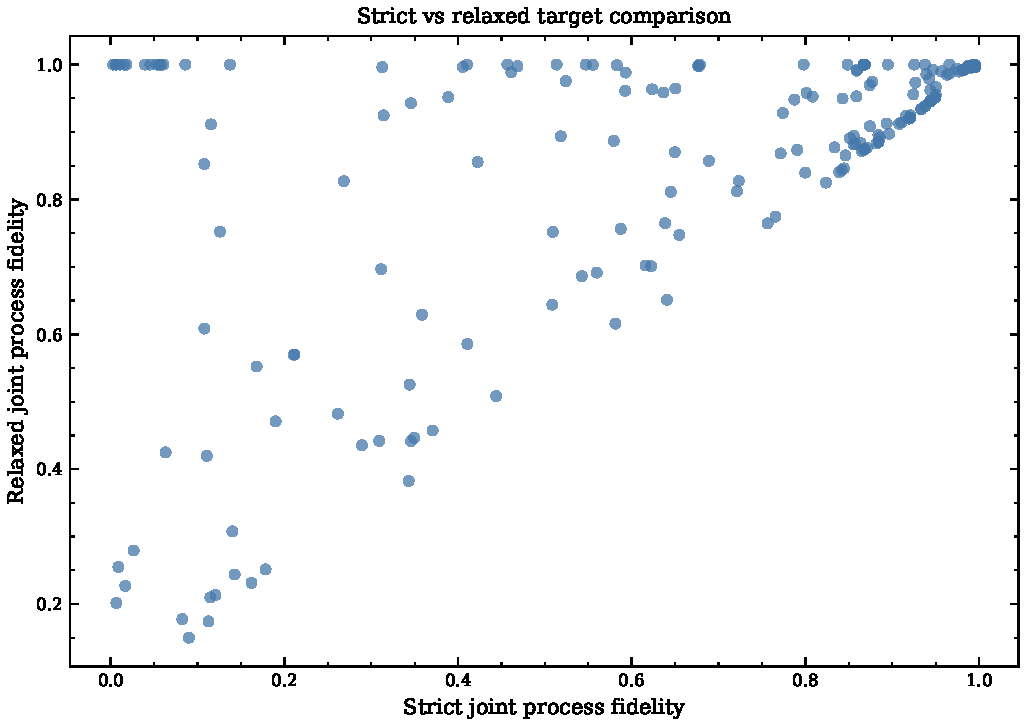
\includegraphics[width=\columnwidth]{../figures/strict_vs_relaxed_comparison.pdf}
\caption{Strict versus relaxed joint process fidelity over the saved dataset.  The strong vertical spread demonstrates that relaxed CPSQR success must not be conflated with strict arbitrary-control success.}
\label{fig:strict_relaxed}
\end{figure}

\section{What Is Ruled Out Versus What Remains Open}
What is ruled out is a strong claim that the tested SQR-style direct or echoed families generically realize arbitrary blockwise SU(2) control on hard target classes.  The random-target ensemble and the stress target both contradict such a claim.

What remains open is whether a true GRAPE benchmark or a richer left/right gauge picture can widen the strict reachable set.  The present evidence says the Gaussian direct family is not uniquely to blame, but it does not amount to a theorem about all possible conditional controls.

\section{Limitations and Future Work}
\subsection{Known limitations}
The main dataset is closed-system and two-level in the optimization loop.  The higher-expressivity benchmark is not a full GRAPE calculation \cite{khaneja2005grape}.  The random-target ensemble is intentionally representative rather than exhaustive.  Finally, the reported CPSQR success depends on the explicit left-$Z$ gauge of Eq.~\eqref{eq:relaxed}; a different relaxation would define a different success class.

\subsection{Suggested improvements}
\begin{enumerate}
\item \textbf{[P1 | HIGH]} Run a true GRAPE benchmark with the same bandwidth and carrier conventions.  This is the clearest next step for separating ansatz failure from deeper controllability limitations.
\item \textbf{[P1 | MEDIUM]} Replay the strict and relaxed highlight cases with $N_{\mathrm{tr}}=3$ and with cavity Kerr enabled.  This would test whether the clean two-level conclusions survive a stronger Hamiltonian.
\item \textbf{[P2 | MEDIUM]} Expand the random-target ensemble and add an explicit right-$Z$ or left/right-$Z$ gauge comparison.  This would sharpen the boundary between CPSQR success and strict SU(2) failure.
\end{enumerate}

\subsection{Open questions}
The strongest open physics question is whether the remaining strict-control failure is fundamentally tied to conditional-$Z$ structure in the dispersive Hamiltonian or whether a sufficiently expressive constrained-control basis can remove it without sacrificing block isolation.

\section{Reproducibility}
The study ships with machine-readable case JSON files, waveform NPZ files, a CSV summary, a JSON summary, a validation report, and an artifact-first notebook.  The primary entry points are:
\begin{enumerate}
\item \path{scripts/run_study.py} to generate or resume the saved result table;
\item \path{scripts/build_reproducibility_notebook.py} to regenerate the notebook;
\item \path{scripts/reproducibility_notebook.ipynb} to inspect or rerun highlight cases interactively.
\end{enumerate}

\section{Conclusion}
The final answers are intentionally narrow.

\begin{enumerate}
\item \textbf{What is convincingly demonstrated.}  Direct Gaussian SQR control can realize strict blockwise targets on restricted subclasses, especially structured and in-plane targets at low active dimension.  Segmented relaxed CPSQR can realize the tested hard targets with essentially perfect relaxed fidelity.
\item \textbf{What is ruled out for the tested waveform classes.}  None of the tested families provides a convincing general strict arbitrary-SU(2) solution for the hard stress and random target classes.
\item \textbf{Whether strict ideal SQR is achievable.}  For arbitrary blockwise control, strict success exists only on a restricted subclass; it is not a generic outcome of the tested families.
\item \textbf{Whether CPSQR is achievable.}  Yes, strongly, under the explicit left-$Z$ blockwise gauge of Eq.~\eqref{eq:relaxed}.  The segmented relaxed family is the clearest positive example.
\item \textbf{Whether success survives full validation.}  The report distinguishes reduced, full-state, and cross-block validation explicitly.  Many relaxed successes survive those checks; many strict failures are exposed only when those checks are enforced.
\item \textbf{What the current best waveform family is.}  For strict control the best family is the direct Gaussian single pulse on the easiest structured cases.  For relaxed CPSQR the best family is the segmented relaxed construction.
\item \textbf{What the minimum convincing duration is.}  The saved strict successes occur already around $|\chi|T/2\pi = 3$ for easy structured cases, while the hard target classes never show a comparably convincing strict threshold in the tested family set.
\item \textbf{What the next most valuable follow-up is.}  Run a true GRAPE benchmark and replay the strict and relaxed highlight cases with $N_{\mathrm{tr}}=3$ or cavity Kerr enabled.
\end{enumerate}

\bibliographystyle{apsrev4-2}
\bibliography{references}

\appendix

\section{Detailed Results and Data}
The saved CSV table contains $114$ family evaluations.  The mean family-level strict and relaxed process fidelities are:
\begin{enumerate}
\item segmented relaxed: $(0.4148,\ 1.0000)$;
\item single-pulse Gaussian: $(0.9176,\ 0.9491)$;
\item independent echo: $(0.5989,\ 0.9286)$;
\item basis-expanded benchmark: $(0.7781,\ 0.8400)$.
\end{enumerate}
The symmetry-constrained echoes are much worse on the saved stress slice and are omitted from the main-text comparison figure for readability.

\section{Reproducibility}
\subsection{Optimized Parameters}
Each case artifact in \texttt{artifacts/cases/} stores the optimized family parameters, the saved strict and relaxed metrics, and the waveform samples used for plotting.

\subsection{Waveform and Pulse Information}
The direct and composite waveform samples are saved as JSON inside each case artifact and as NPZ files in \texttt{artifacts/waveforms/}.  The main-text waveform examples are reproduced from these files.

\subsection{Gate Sequence and Decomposition}
The saved metadata records the control-family construction, active duration, total gate duration, segment durations, and any inserted $X_\pi$ pulses.

\subsection{Modeling and Simulation Assumptions}
The artifact metadata also records the target class, model variant, $N_{\mathrm{active}}$, the selected duration parameter $|\chi|T/2\pi$, and whether the run used the \texttt{chi\_only} or \texttt{chi\_plus\_chiprime} model.

\subsection{Reproduction Procedure}
\begin{enumerate}
\item Run \texttt{python} on \path{scripts/run_study.py} to regenerate or resume the saved result table.
\item Run \texttt{python} on \path{scripts/build_reproducibility_notebook.py} to regenerate the notebook.
\item Open \path{scripts/reproducibility_notebook.ipynb} for artifact-first inspection or to rerun selected cases.
\item Compare the recreated figures in \path{figures/} against the saved PDF/PNG outputs.
\end{enumerate}

\subsection{Saved Artifacts}
The core machine-readable outputs are:
\begin{enumerate}
\item \texttt{data/study\_results.csv};
\item \texttt{data/study\_results.json};
\item \texttt{data/study\_summary.json};
\item \texttt{data/validation\_summary.json};
\item per-case JSON files in \texttt{artifacts/cases/};
\item waveform NPZ files in \texttt{artifacts/waveforms/}.
\end{enumerate}

\end{document}
